\chapter{ترکیبیات}

\index{ترکیبیات}

\key{ترکیبیات} روش‌های شمارش ترکیب‌های اشیاء را بررسی می‌کند.
معمولاً هدف یافتن روشی برای شمارش کارآمد ترکیب‌ها
بدون تولید مجزای هر ترکیب است.

به عنوان مثال، مسئله شمارش تعداد روش‌های نمایش
یک عدد صحیح $n$ به صورت مجموعی از اعداد صحیح مثبت را در نظر بگیرید.
به عنوان مثال، ۸ روش نمایش برای عدد $4$ وجود دارد:
\begin{multicols}{2}
\begin{itemize}
\item $1+1+1+1$
\item $1+1+2$
\item $1+2+1$
\item $2+1+1$
\item $2+2$
\item $3+1$
\item $1+3$
\item $4$
\end{itemize}
\end{multicols}

یک مسئله ترکیبیاتی اغلب می‌تواند با استفاده از یک تابع بازگشتی حل شود.
در این مسئله، می‌توانیم تابع $f(n)$ را تعریف کنیم
که تعداد روش‌های نمایش $n$ را به دست می‌دهد.
به عنوان مثال، مطابق با مثال بالا $f(4)=8$ است.
مقادیر این تابع را می‌توان به صورت بازگشتی به روش زیر محاسبه کرد:
\begin{equation*}
    f(n) = \begin{cases}
               1               & n = 0\\
               f(0)+f(1)+\cdots+f(n-1) & n > 0\\
           \end{cases}
\end{equation*}
حالت پایه $f(0)=1$ است،
زیرا مجموع تهی بیانگر عدد 0 است.
سپس، اگر $n>0$ باشد، تمام روش‌های انتخاب عدد اول مجموع را در نظر می‌گیریم.
اگر عدد اول $k$ باشد،
$f(n-k)$ روش نمایش برای بخش باقیمانده مجموع وجود دارد.
بنابراین، مجموع تمام مقادیر به فرم $f(n-k)$ را محاسبه می‌کنیم که در آن $k<n$ است.

نخستین مقادیر این تابع عبارتند از:
\[
\begin{array}{lcl}
f(0) & = & 1 \\
f(1) & = & 1 \\
f(2) & = & 2 \\
f(3) & = & 4 \\
f(4) & = & 8 \\
\end{array}
\]

گاهی می‌توان فرمول بازگشتی را با یک فرمول بسته جایگزین کرد.
در این مسئله،
\[
f(n)=2^{n-1},
\]
که بر اساس این واقعیت است که $n-1$ موقعیت ممکن برای علامت‌های + در مجموع وجود دارد
و ما می‌توانیم هر زیرمجموعه‌ای از آن‌ها را انتخاب کنیم.

\section{ضرایب دوجمله‌ای}

\index{ضریب دوجمله‌ای}

\key{ضریب دوجمله‌ای} ${n \choose k}$ برابر با تعداد روش‌هایی است
که می‌توان یک زیرمجموعه $k$ عضوی را از یک مجموعه $n$ عضوی انتخاب کرد.
برای مثال، ${5 \choose 3}=10$،
زیرا مجموعه $\{1,2,3,4,5\}$
دارای ۱۰ زیرمجموعه ۳ عضوی است:
\[ \{1,2,3\}, \{1,2,4\}, \{1,2,5\}, \{1,3,4\}, \{1,3,5\}, 
\{1,4,5\}, \{2,3,4\}, \{2,3,5\}, \{2,4,5\}, \{3,4,5\} \]

\subsubsection{فرمول ۱}

ضرایب دوجمله‌ای را می‌توان به صورت بازگشتی به صورت زیر محاسبه کرد:

\[
{n \choose k}  =  {n-1 \choose k-1} + {n-1 \choose k}
\]

ایده این است که یک عنصر $x$ را در مجموعه تثبیت کنیم.
اگر $x$ در زیرمجموعه گنجانده شود،
باید $k-1$ عنصر را از $n-1$ عنصر انتخاب کنیم،
و اگر $x$ در زیرمجموعه گنجانده نشود،
باید $k$ عنصر را از $n-1$ عنصر انتخاب کنیم.

حالت‌های پایه برای بازگشت عبارتند از:
\[
{n \choose 0}  =  {n \choose n} = 1,
\]
زیرا همواره دقیقاً یک روش برای ساخت زیرمجموعه تهی
و یک زیرمجموعه شامل تمام عناصر وجود دارد.

\subsubsection{فرمول ۲}

روش دیگر برای محاسبه ضرایب دوجمله‌ای به صورت زیر است:
\[
{n \choose k}  =  \frac{n!}{k!(n-k)!}.
\]

$n!$ جایگشت برای $n$ عنصر وجود دارد.
تمام جایگشت‌ها را بررسی می‌کنیم و همواره
$k$ عنصر اول جایگشت را در زیرمجموعه قرار می‌دهیم.
از آنجا که ترتیب عناصر در داخل زیرمجموعه
و خارج از آن اهمیتی ندارد،
نتیجه بر $k!$ و $(n-k)!$ تقسیم می‌شود.

\subsubsection{ویژگی‌ها}

برای ضرایب دوجمله‌ای،
\[
{n \choose k}  =  {n \choose n-k},
\]
چرا که در واقع یک مجموعه از $n$ عنصر را به
دو زیرمجموعه تقسیم می‌کنیم: اولی شامل $k$ عنصر
و دومی شامل $n-k$ عنصر است.

مجموع ضرایب دوجمله‌ای برابر است با:
\[
{n \choose 0}+{n \choose 1}+{n \choose 2}+\ldots+{n \choose n}=2^n.
\]

علت نام‌گذاری «ضریب دوجمله‌ای»
هنگام به توان $n$ رساندن دوجمله‌ای $(a+b)$ مشخص می‌شود:

\[ (a+b)^n =
{n \choose 0} a^n b^0 + 
{n \choose 1} a^{n-1} b^1 +
\ldots + 
{n \choose n-1} a^1 b^{n-1} +
{n \choose n} a^0 b^n. \]

\index{مثلث پاسکال}

ضرایب دوجمله‌ای در \key{مثلث پاسکال} نیز ظاهر می‌شوند،
جایی که هر مقدار برابر با مجموع دو مقدار
بالای خود است:
\begin{center}
\begin{tikzpicture}{0.9}
\node at (0,0) {1};
\node at (-0.5,-0.5) {1};
\node at (0.5,-0.5) {1};
\node at (-1,-1) {1};
\node at (0,-1) {2};
\node at (1,-1) {1};
\node at (-1.5,-1.5) {1};
\node at (-0.5,-1.5) {3};
\node at (0.5,-1.5) {3};
\node at (1.5,-1.5) {1};
\node at (-2,-2) {1};
\node at (-1,-2) {4};
\node at (0,-2) {6};
\node at (1,-2) {4};
\node at (2,-2) {1};
\node at (-2,-2.5) {$\ldots$};
\node at (-1,-2.5) {$\ldots$};
\node at (0,-2.5) {$\ldots$};
\node at (1,-2.5) {$\ldots$};
\node at (2,-2.5) {$\ldots$};
\end{tikzpicture}
\end{center}

\subsubsection{جعبه‌ها و توپ‌ها}

«جعبه‌ها و توپ‌ها» یک مدل کاربردی است
که در آن تعداد روش‌های قرار دادن
$k$ توپ در $n$ جعبه را می‌شماریم.
سه حالت را در نظر می‌گیریم:

\textit{حالت ۱}: هر جعبه می‌تواند حداکثر
شامل یک توپ باشد.
به عنوان مثال، وقتی $n=5$ و $k=2$ باشد،
۱۰ روش وجود دارد:

\begin{center}
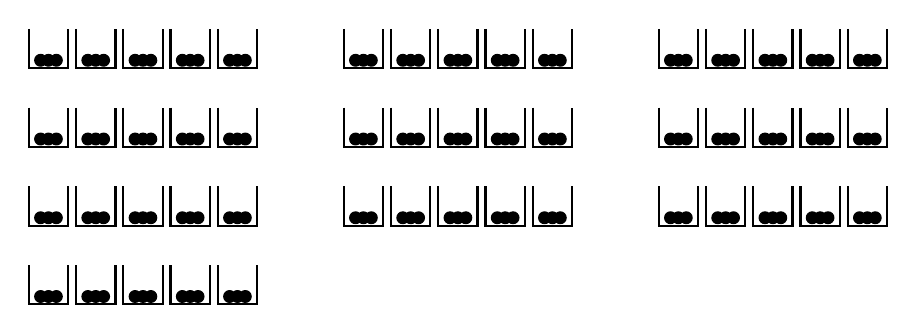
\begin{tikzpicture}[scale=0.5]
\newcommand\lax[3]{
\path[draw,thick,-] (#1-0.5,#2+0.5) -- (#1-0.5,#2-0.5) --
                    (#1+0.5,#2-0.5) -- (#1+0.5,#2+0.5);
\ifthenelse{\equal{#3}{1}}{\draw[fill=black] (#1,#2-0.3) circle (0.15);}{}
\ifthenelse{\equal{#3}{2}}{\draw[fill=black] (#1-0.2,#2-0.3) circle (0.15);}{}
\ifthenelse{\equal{#3}{2}}{\draw[fill=black] (#1+0.2,#2-0.3) circle (0.15);}{}
}
\newcommand\laa[7]{
    \lax{#1}{#2}{#3}
    \lax{#1+1.2}{#2}{#4}
    \lax{#1+2.4}{#2}{#5}
    \lax{#1+3.6}{#2}{#6}
    \lax{#1+4.8}{#2}{#7}
}

\laa{0}{0}{1}{1}{0}{0}{0}
\laa{0}{-2}{1}{0}{1}{0}{0}
\laa{0}{-4}{1}{0}{0}{1}{0}
\laa{0}{-6}{1}{0}{0}{0}{1}
\laa{8}{0}{0}{1}{1}{0}{0}
\laa{8}{-2}{0}{1}{0}{1}{0}
\laa{8}{-4}{0}{1}{0}{0}{1}
\laa{16}{0}{0}{0}{1}{1}{0}
\laa{16}{-2}{0}{0}{1}{0}{1}
\laa{16}{-4}{0}{0}{0}{1}{1}

\end{tikzpicture}
\end{center}

در این حالت، پاسخ مستقیماً ضریب
دوجمله‌ای ${n \choose k}$ است.

\textit{حالت ۲}: یک جعبه می‌تواند شامل چند توپ باشد.
به عنوان مثال، وقتی $n=5$ و $k=2$ باشد،
۱۵ روش وجود دارد:

\begin{center}
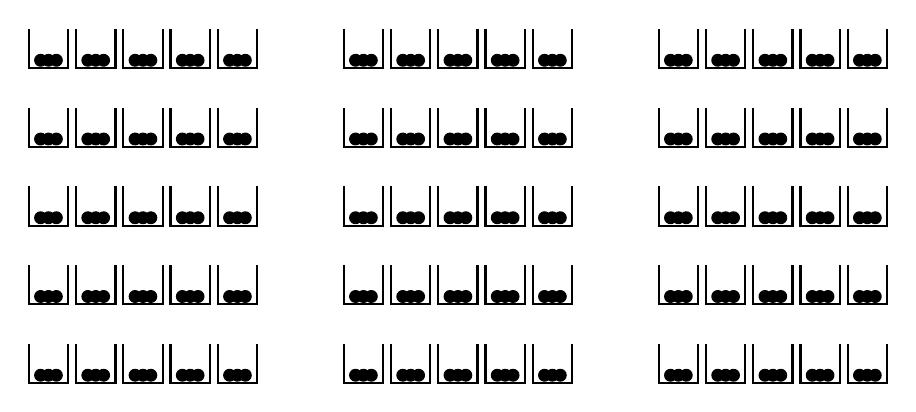
\begin{tikzpicture}[scale=0.5]
\newcommand\lax[3]{
\path[draw,thick,-] (#1-0.5,#2+0.5) -- (#1-0.5,#2-0.5) --
                    (#1+0.5,#2-0.5) -- (#1+0.5,#2+0.5);
\ifthenelse{\equal{#3}{1}}{\draw[fill=black] (#1,#2-0.3) circle (0.15);}{}
\ifthenelse{\equal{#3}{2}}{\draw[fill=black] (#1-0.2,#2-0.3) circle (0.15);}{}
\ifthenelse{\equal{#3}{2}}{\draw[fill=black] (#1+0.2,#2-0.3) circle (0.15);}{}
}
\newcommand\laa[7]{
    \lax{#1}{#2}{#3}
    \lax{#1+1.2}{#2}{#4}
    \lax{#1+2.4}{#2}{#5}
    \lax{#1+3.6}{#2}{#6}
    \lax{#1+4.8}{#2}{#7}
}

\laa{0}{0}{2}{0}{0}{0}{0}
\laa{0}{-2}{1}{1}{0}{0}{0}
\laa{0}{-4}{1}{0}{1}{0}{0}
\laa{0}{-6}{1}{0}{0}{1}{0}
\laa{0}{-8}{1}{0}{0}{0}{1}
\laa{8}{0}{0}{2}{0}{0}{0}
\laa{8}{-2}{0}{1}{1}{0}{0}
\laa{8}{-4}{0}{1}{0}{1}{0}
\laa{8}{-6}{0}{1}{0}{0}{1}
\laa{8}{-8}{0}{0}{2}{0}{0}
\laa{16}{0}{0}{0}{1}{1}{0}
\laa{16}{-2}{0}{0}{1}{0}{1}
\laa{16}{-4}{0}{0}{0}{2}{0}
\laa{16}{-6}{0}{0}{0}{1}{1}
\laa{16}{-8}{0}{0}{0}{0}{2}

\end{tikzpicture}
\end{center}

فرایند قرار دادن توپ‌ها در جعبه‌ها را می‌توان با رشته‌ای شامل نمادهای «o» و «$\rightarrow$» نمایش داد. ابتدا فرض کنید در چپ‌ترین جعبه ایستاده‌ایم. نماد «o» یعنی یک توپ در جعبه فعلی بگذار، و نماد «$\rightarrow$» یعنی به جعبه بعدی در سمت راست برو.

با این نمایش، هر جواب رشته‌ای است شامل $k$ بار نماد «o» و $n-1$ بار نماد «$\rightarrow$». برای نمونه، جواب بالا-راست در تصویر بالا معادل رشته «$\rightarrow$ $\rightarrow$ o $\rightarrow$ o $\rightarrow$» است. بنابراین، تعداد جواب‌ها برابر است با:
${k+n-1 \choose k}$.

\textit{سناریوی ۳}: هر جعبه حداکثر یک توپ دارد، بعلاوه هیچ دو جعبه مجاوری نباید همزمان توپ داشته باشند. برای نمونه، به ازای $n=5$ و $k=2$، تعداد ۶ جواب وجود دارد:

\begin{center}
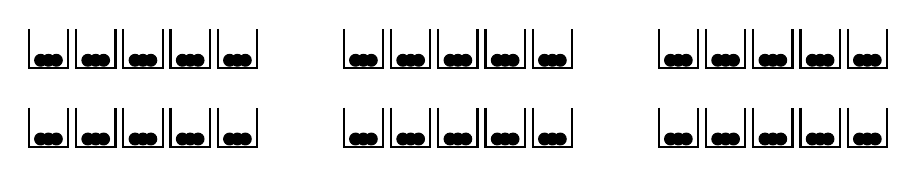
\begin{tikzpicture}[scale=0.5]
\newcommand\lax[3]{
\path[draw,thick,-] (#1-0.5,#2+0.5) -- (#1-0.5,#2-0.5) --
                    (#1+0.5,#2-0.5) -- (#1+0.5,#2+0.5);
\ifthenelse{\equal{#3}{1}}{\draw[fill=black] (#1,#2-0.3) circle (0.15);}{}
\ifthenelse{\equal{#3}{2}}{\draw[fill=black] (#1-0.2,#2-0.3) circle (0.15);}{}
\ifthenelse{\equal{#3}{2}}{\draw[fill=black] (#1+0.2,#2-0.3) circle (0.15);}{}
}
\newcommand\laa[7]{
    \lax{#1}{#2}{#3}
    \lax{#1+1.2}{#2}{#4}
    \lax{#1+2.4}{#2}{#5}
    \lax{#1+3.6}{#2}{#6}
    \lax{#1+4.8}{#2}{#7}
}

\laa{0}{0}{1}{0}{1}{0}{0}
\laa{0}{-2}{1}{0}{0}{1}{0}
\laa{8}{0}{1}{0}{0}{0}{1}
\laa{8}{-2}{0}{1}{0}{1}{0}
\laa{16}{0}{0}{1}{0}{0}{1}
\laa{16}{-2}{0}{0}{1}{0}{1}
\end{tikzpicture}
\end{center}

در این سناریو فرض کنید $k$ توپ ابتدا درون جعبه‌ها قرار دارند و بین هر دو جعبه مجاور یک جعبه خالی قرار گرفته است. کار باقی‌مانده انتخاب جایگاه برای جعبه‌های خالی باقی‌مانده است. تعداد $n-2k+1$ جعبه خالی و $k+1$ موقعیت ممکن برای قرار دادن آن‌ها داریم. بنابراین با فرمول سناریوی ۲، تعداد جواب‌ها برابر است با:
${n-k+1 \choose n-2k+1}$.

\subsubsection{ضرایب چندجمله‌ای}

\index{ضریب چندجمله‌ای}

\key{ضریب چندجمله‌ای}
\[ {n \choose k_1,k_2,\ldots,k_m} = \frac{n!}{k_1! k_2! \cdots k_m!}, \]
برابر با تعداد روش‌هایی است که
می‌توان $n$ عنصر را به زیرمجموعه‌هایی
با اندازه‌های $k_1,k_2,\ldots,k_m$ تقسیم کرد،
به طوری که $k_1+k_2+\cdots+k_m=n$ باشد.
ضرایب چندجمله‌ای را می‌توان تعمیم
ضرایب دوجمله‌ای دانست؛
اگر $m=2$ باشد، فرمول بالا
با فرمول ضریب دوجمله‌ای مطابقت دارد.

\section{اعداد کاتالان}

\index{عدد کاتالان}

\key{عدد کاتالان}
%\footnote{E. C. Catalan (1814--1894) was a Belgian mathematician.}
$C_n$ برابر با
تعداد عبارت‌های پرانتزگذاری معتبری است که از
$n$ پرانتز باز و $n$ پرانتز بسته تشکیل شده‌اند.

به عنوان مثال، $C_3=5$ است، زیرا
می‌توان عبارت‌های پرانتزی زیر را با استفاده از سه
پرانتز باز و بسته ساخت:

\begin{itemize}[noitemsep]
\item \texttt{()()()}
\item \texttt{(())()}
\item \texttt{()(())}
\item \texttt{((()))}
\item \texttt{(()())}
\end{itemize}

\subsubsection{عبارت‌های پرانتزی}

\index{عبارت پرانتزی}

یک \emph{عبارت پرانتزی معتبر} دقیقا چیست؟
قوانین زیر تمام
عبارت‌های پرانتزی معتبر را به‌طور دقیق تعریف می‌کنند:

\begin{itemize}
\item یک عبارت پرانتزی خالی معتبر است.
\item اگر عبارت $A$ معتبر باشد،
آنگاه عبارت
\texttt{(}$A$\texttt{)} نیز معتبر است.
\item اگر عبارت‌های $A$ و $B$ معتبر باشند،
آنگاه عبارت $AB$ نیز معتبر است.
\end{itemize}

روش دیگر برای توصیف عبارت‌های پرانتزی
معتبر این است که اگر
هر پیشوندی از چنین عبارتی را انتخاب کنیم،
باید حداقل به تعداد پرانتزهای بسته، پرانتز باز
داشته باشد.
علاوه بر این، کل عبارت باید
دارای تعداد برابری از پرانتزهای باز و بسته
باشد.

\subsubsection{فرمول ۱}

اعداد کاتالان را می‌توان با استفاده از این فرمول محاسبه کرد:
\[ C_n = \sum_{i=0}^{n-1} C_{i} C_{n-i-1}.\]

این مجموع، حالات تقسیم
عبارت به دو بخش را بررسی می‌کند
به طوری که هر دو بخش، عبارت‌های
معتبری باشند و بخش اول تا حد امکان کوتاه
اما غیرخالی باشد.
به ازای هر $i$، بخش اول شامل $i+1$ جفت
پرانتز است و تعداد عبارت‌ها
حاصل‌ضرب مقادیر زیر است:

\begin{itemize}
\item $C_{i}$: تعداد روش‌های ساخت یک عبارت
با استفاده از پرانتزهای بخش اول،
بدون در نظر گرفتن بیرونی‌ترین پرانتزها
\item $C_{n-i-1}$: تعداد روش‌های ساخت یک
عبارت با استفاده از پرانتزهای بخش دوم
\end{itemize}

حالت پایه $C_0=1$ است،
زیرا می‌توان با استفاده از صفر جفت پرانتز، یک عبارت پرانتزی
خالی ساخت.

\subsubsection{فرمول ۲}

اعداد کاتالان را می‌توان
با استفاده از ضرایب دوجمله‌ای نیز محاسبه کرد:
\[ C_n = \frac{1}{n+1} {2n \choose n}\]
این فرمول را می‌توان به صورت زیر توضیح داد:

در مجموع ${2n \choose n}$ روش
برای ساخت یک عبارت پرانتزی (نه لزوماً معتبر)
شامل $n$ پرانتز باز و $n$ پرانتز بسته وجود دارد.
بیایید تعداد عباراتی از این دست را که معتبر \emph{نیستند}
محاسبه کنیم.

اگر یک عبارت پرانتزی معتبر نباشد،
باید دارای پیشوندی باشد که در آن
تعداد پرانتزهای بسته از تعداد پرانتزهای باز بیشتر شود.
ایده این است که جهت هر پرانتز متعلق به چنین پیشوندی را معکوس کنیم.
برای نمونه، عبارت
\texttt{())()(} شامل پیشوند \texttt{())} است،
و پس از معکوس کردن این پیشوند،
عبارت به شکل \texttt{)((()(} درمی‌آید.

عبارت حاصل از $n+1$
پرانتز باز و $n-1$ پرانتز بسته تشکیل شده است.
تعداد چنین عباراتی برابر با ${2n \choose n+1}$ است،
که معادل تعداد عبارات پرانتزی نامعتبر می‌باشد.
بنابراین، تعداد عبارات پرانتزی معتبر
را می‌توان با فرمول زیر محاسبه کرد:
\[{2n \choose n}-{2n \choose n+1} = {2n \choose n} - \frac{n}{n+1} {2n \choose n} = \frac{1}{n+1} {2n \choose n}.\]

\subsubsection{شمارش درخت‌ها}

اعداد کاتالان با درخت‌ها نیز مرتبط هستند:

\begin{itemize}
\item $C_n$ درخت دودویی با $n$ رأس وجود دارد
\item $C_{n-1}$ درخت ریشه‌دار با $n$ رأس وجود دارد
\end{itemize}
\noindent
به عنوان مثال، برای $C_3=5$، درخت‌های دودویی عبارتند از:

\begin{center}
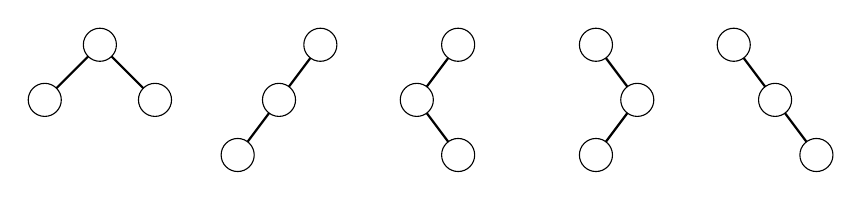
\begin{tikzpicture}[scale=0.7]
\path[draw,thick,-] (0,0) -- (-1,-1);
\path[draw,thick,-] (0,0) -- (1,-1);
\draw[fill=white] (0,0) circle (0.3);
\draw[fill=white] (-1,-1) circle (0.3);
\draw[fill=white] (1,-1) circle (0.3);

\path[draw,thick,-] (4,0) -- (4-0.75,-1) -- (4-1.5,-2);
\draw[fill=white] (4,0) circle (0.3);
\draw[fill=white] (4-0.75,-1) circle (0.3);
\draw[fill=white] (4-1.5,-2) circle (0.3);

\path[draw,thick,-] (6.5,0) -- (6.5-0.75,-1) -- (6.5-0,-2);
\draw[fill=white] (6.5,0) circle (0.3);
\draw[fill=white] (6.5-0.75,-1) circle (0.3);
\draw[fill=white] (6.5-0,-2) circle (0.3);

\path[draw,thick,-] (9,0) -- (9+0.75,-1) -- (9-0,-2);
\draw[fill=white] (9,0) circle (0.3);
\draw[fill=white] (9+0.75,-1) circle (0.3);
\draw[fill=white] (9-0,-2) circle (0.3);

\path[draw,thick,-] (11.5,0) -- (11.5+0.75,-1) -- (11.5+1.5,-2);
\draw[fill=white] (11.5,0) circle (0.3);
\draw[fill=white] (11.5+0.75,-1) circle (0.3);
\draw[fill=white] (11.5+1.5,-2) circle (0.3);
\end{tikzpicture}
\end{center}
و درخت‌های ریشه‌دار عبارتند از:
\begin{center}
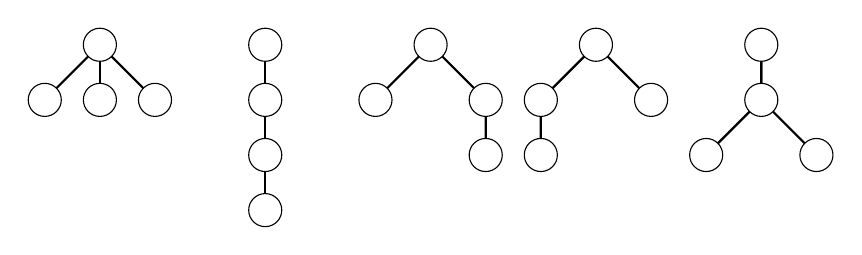
\begin{tikzpicture}[scale=0.7]
\path[draw,thick,-] (0,0) -- (-1,-1);
\path[draw,thick,-] (0,0) -- (0,-1);
\path[draw,thick,-] (0,0) -- (1,-1);
\draw[fill=white] (0,0) circle (0.3);
\draw[fill=white] (-1,-1) circle (0.3);
\draw[fill=white] (0,-1) circle (0.3);
\draw[fill=white] (1,-1) circle (0.3);

\path[draw,thick,-] (3,0) -- (3,-1) -- (3,-2) -- (3,-3);
\draw[fill=white] (3,0) circle (0.3);
\draw[fill=white] (3,-1) circle (0.3);
\draw[fill=white] (3,-2) circle (0.3);
\draw[fill=white] (3,-3) circle (0.3);

\path[draw,thick,-] (6+0,0) -- (6-1,-1);
\path[draw,thick,-] (6+0,0) -- (6+1,-1) -- (6+1,-2);
\draw[fill=white] (6+0,0) circle (0.3);
\draw[fill=white] (6-1,-1) circle (0.3);
\draw[fill=white] (6+1,-1) circle (0.3);
\draw[fill=white] (6+1,-2) circle (0.3);

\path[draw,thick,-] (9+0,0) -- (9+1,-1);
\path[draw,thick,-] (9+0,0) -- (9-1,-1) -- (9-1,-2);
\draw[fill=white] (9+0,0) circle (0.3);
\draw[fill=white] (9+1,-1) circle (0.3);
\draw[fill=white] (9-1,-1) circle (0.3);
\draw[fill=white] (9-1,-2) circle (0.3);

\path[draw,thick,-] (12+0,0) -- (12+0,-1) -- (12-1,-2);
\path[draw,thick,-] (12+0,0) -- (12+0,-1) -- (12+1,-2);
\draw[fill=white] (12+0,0) circle (0.3);
\draw[fill=white] (12+0,-1) circle (0.3);
\draw[fill=white] (12-1,-2) circle (0.3);
\draw[fill=white] (12+1,-2) circle (0.3);

\end{tikzpicture}
\end{center}

\section{اصل شمول و عدم شمول}

\index{شمول و عدم شمول}

\key{اصل شمول و عدم شمول} روشی برای
شمارش اندازه اجتماع مجموعه‌هاست،
وقتی اندازه اشتراک‌ها معلوم باشد (و برعکس).
نمونه ساده فرمول:
\[ |A \cup B| = |A| + |B| - |A \cap B|,\]
که $A$ و $B$ مجموعه هستند و $|X|$
اندازه $X$ را نشان می‌دهد.
نمایش فرمول:

\begin{center}
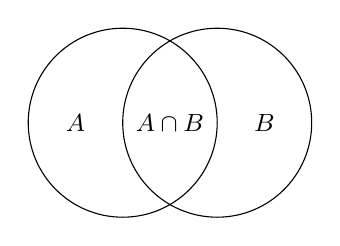
\begin{tikzpicture}[scale=0.8]

\draw (0,0) circle (1.5);
\draw (1.5,0) circle (1.5);

\node at (-0.75,0) {\small $A$};
\node at (2.25,0) {\small $B$};
\node at (0.75,0) {\small $A \cap B$};

\end{tikzpicture}
\end{center}

هدف: محاسبه اندازه اجتماع $A \cup B$؛
هم‌ارز مساحت ناحیه درون حداقل یک دایره.
تصویر نشان می‌دهد: مساحت $A \cup B$ برابر
مجموع مساحت‌های $A$ و $B$ منهای
مساحت $A \cap B$.

ایده برای تعداد بیشتر مجموعه‌ها هم کار می‌کند.
برای سه مجموعه، فرمول شمول و عدم شمول:
\[ |A \cup B \cup C| = |A| + |B| + |C| - |A \cap B|  - |A \cap C|  - |B \cap C| + |A \cap B \cap C| \]
تصویر متناظر:

\begin{center}
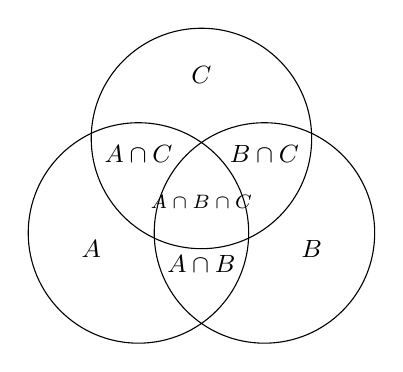
\begin{tikzpicture}[scale=0.8]

\draw (0,0) circle (1.75);
\draw (2,0) circle (1.75);
\draw (1,1.5) circle (1.75);

\node at (-0.75,-0.25) {\small $A$};
\node at (2.75,-0.25) {\small $B$};
\node at (1,2.5) {\small $C$};
\node at (1,-0.5) {\small $A \cap B$};
\node at (0,1.25) {\small $A \cap C$};
\node at (2,1.25) {\small $B \cap C$};
\node at (1,0.5) {\scriptsize $A \cap B \cap C$};

\end{tikzpicture}
\end{center}

حالت کلی: محاسبه اندازه اجتماع
$X_1 \cup X_2 \cup \cdots \cup X_n$
با پیمایش تمام اشتراک‌های ممکن از زیرمجموعه‌های
$X_1,X_2,\ldots,X_n$.
اگر اشتراک شامل تعداد فردی مجموعه باشد،
اندازه‌اش به جواب اضافه می‌شود؛
در غیر این صورت، از جواب کم می‌شود.

توجه کنید که فرمول‌های مشابهی نیز برای محاسبه اندازه اشتراک بر اساس اندازه اجتماع‌ها وجود دارد. به عنوان مثال،
\[ |A \cap B| = |A| + |B| - |A \cup B|\]
و
\[ |A \cap B \cap C| = |A| + |B| + |C| - |A \cup B|  - |A \cup C|  - |B \cup C| + |A \cup B \cup C| .\]

\subsubsection{پریش‌ها}

\index{پریش}

به عنوان مثال، بیایید تعداد \key{پریش‌های} (derangements) اعضای مجموعه $\{1,2,\ldots,n\}$ را بشماریم؛ یعنی جایگشت‌هایی که در آن‌ها هیچ عنصری در جایگاه اصلی خود باقی نمی‌ماند.
برای نمونه، وقتی $n=3$ باشد، دو پریش وجود دارد: $(2,3,1)$ و $(3,1,2)$.

یک روش برای حل مسئله، استفاده از اصل شمول و عدم شمول است.
فرض کنید $X_k$ مجموعه جایگشت‌هایی باشد که عنصر $k$ در موقعیت $k$ قرار دارد.
برای مثال، وقتی $n=3$ باشد، این مجموعه‌ها به صورت زیر هستند:
\[
\begin{array}{lcl}
X_1 & = & \{(1,2,3),(1,3,2)\} \\
X_2 & = & \{(1,2,3),(3,2,1)\} \\
X_3 & = & \{(1,2,3),(2,1,3)\} \\
\end{array}
\]
با استفاده از این مجموعه‌ها، تعداد پریش‌ها برابر است با
\[ n! - |X_1 \cup X_2 \cup \cdots \cup X_n|, \]
بنابراین کافی است اندازه اجتماع محاسبه شود.
با استفاده از اصل شمول و عدم شمول، مسئله به محاسبه اندازه اشتراک‌ها تبدیل می‌شود که به صورت کارآمد قابل انجام است.
برای نمونه، زمانی که $n=3$ باشد، اندازه $|X_1 \cup X_2 \cup X_3|$ برابر است با
\[
\begin{array}{lcl}
 & & |X_1| + |X_2| + |X_3| - |X_1 \cap X_2|  - |X_1 \cap X_3|  - |X_2 \cap X_3| + |X_1 \cap X_2 \cap X_3| \\
 & = & 2+2+2-1-1-1+1 \\
 & = & 4, \\
\end{array}
\]
بنابراین تعداد جواب‌ها $3!-4=2$ است.

مشخص می‌شود که این مسئله را می‌توان بدون استفاده از اصل شمول و عدم شمول نیز حل کرد.
فرض کنید $f(n)$ نشان‌دهنده تعداد پریش‌ها برای $\{1,2,\ldots,n\}$ باشد. می‌توان از رابطه بازگشتی زیر استفاده کرد:

\begin{equation*}
    f(n) = \begin{cases}
               0               & n = 1\\
               1               & n = 2\\
               (n-1)(f(n-2) + f(n-1)) & n>2 \\
           \end{cases}
\end{equation*}

این رابطه را می‌توان با بررسی حالت‌های ممکن برای تغییر جایگاه عنصر ۱ به دست آورد.
تعداد $n-1$ روش برای انتخاب عنصر $x$ که جایگزین عنصر ۱ می‌شود وجود دارد.
در هر یک از این انتخاب‌ها، دو حالت ممکن است رخ دهد:

\textit{حالت ۱:} عنصر $x$ نیز با عنصر ۱ جایگزین شود.
پس از این، وظیفه باقی‌مانده ساخت یک پریش از $n-2$ عنصر است.

\textit{حالت ۲:} عنصر $x$ با عنصری غیر از ۱ جایگزین شود.
اکنون باید یک پریش از $n-1$ عنصر بسازیم، زیرا نمی‌توانیم عنصر $x$ را با عنصر ۱ جایگزین کنیم، و تمام عناصر دیگر نیز باید تغییر موقعیت دهند.

\section{لم برنساید}

\index{لم برنساید}

\key{لم برنساید}
%\footnote{در واقع برنساید این لم را کشف نکرد؛ او صرفاً آن را در کتاب خود \cite{bur97} ذکر کرد.}
می‌تواند برای شمارش تعداد ترکیب‌ها به کار رود، به‌گونه‌ای که برای هر گروه از ترکیب‌های متقارن فقط یک نماینده شمرده شود.
لم برنساید بیان می‌کند که تعداد ترکیب‌ها برابر است با:
\[\sum_{k=1}^n \frac{c(k)}{n},\]
که در آن $n$ روش برای تغییر وضعیت یک ترکیب وجود دارد، و $c(k)$ تعداد ترکیب‌هایی است که با اعمال روش $k$ام بدون تغییر باقی می‌مانند.

به عنوان مثال، تعداد گردنبندهای با $n$ مروارید را محاسبه می‌کنیم، که در آن هر مروارید $m$ رنگ ممکن دارد. دو گردنبند متقارن‌اند اگر با دوران مشابه یکدیگر شوند.
برای مثال، گردنبند
\begin{center}
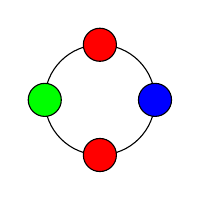
\begin{tikzpicture}[scale=0.7]
\draw[fill=white] (0,0) circle (1);
\draw[fill=red] (0,1) circle (0.3);
\draw[fill=blue] (1,0) circle (0.3);
\draw[fill=red] (0,-1) circle (0.3);
\draw[fill=green] (-1,0) circle (0.3);
\end{tikzpicture}
\end{center}
گردنبندهای متقارن زیر را دارد:
\begin{center}
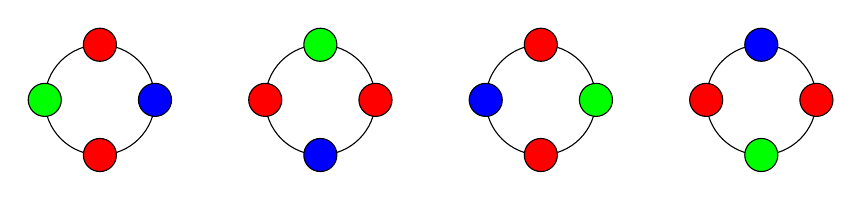
\begin{tikzpicture}[scale=0.7]
\draw[fill=white] (0,0) circle (1);
\draw[fill=red] (0,1) circle (0.3);
\draw[fill=blue] (1,0) circle (0.3);
\draw[fill=red] (0,-1) circle (0.3);
\draw[fill=green] (-1,0) circle (0.3);

\draw[fill=white] (4,0) circle (1);
\draw[fill=green] (4+0,1) circle (0.3);
\draw[fill=red] (4+1,0) circle (0.3);
\draw[fill=blue] (4+0,-1) circle (0.3);
\draw[fill=red] (4+-1,0) circle (0.3);

\draw[fill=white] (8,0) circle (1);
\draw[fill=red] (8+0,1) circle (0.3);
\draw[fill=green] (8+1,0) circle (0.3);
\draw[fill=red] (8+0,-1) circle (0.3);
\draw[fill=blue] (8+-1,0) circle (0.3);

\draw[fill=white] (12,0) circle (1);
\draw[fill=blue] (12+0,1) circle (0.3);
\draw[fill=red] (12+1,0) circle (0.3);
\draw[fill=green] (12+0,-1) circle (0.3);
\draw[fill=red] (12+-1,0) circle (0.3);
\end{tikzpicture}
\end{center}
$n$ روش برای تغییر وضعیت گردنبند وجود دارد، زیرا می‌توان آن را $0,1,\ldots,n-1$ گام در جهت عقربه‌های ساعت چرخاند.
اگر تعداد گام‌ها 0 باشد، همه $m^n$ گردنبند یکسان می‌مانند، و اگر تعداد گام‌ها 1 باشد، تنها $m$ گردنبندی که در آن‌ها همه مرواریدها یک‌رنگ هستند بدون تغییر باقی می‌مانند.

به طور کلی‌تر، وقتی تعداد گام‌ها $k$ است، در مجموع
\[m^{\textrm{gcd}(k,n)}\]
گردنبند بدون تغییر باقی می‌مانند، که $\textrm{gcd}(k,n)$ ب.م.م $k$ و $n$ است.
دلیل این است که بلوک‌هایی از مرواریدها با اندازه $\textrm{gcd}(k,n)$ جایگزین یکدیگر می‌شوند.
بنابراین، بر طبق لم برنساید، تعداد گردنبندها برابر است با:
\[\sum_{i=0}^{n-1} \frac{m^{\textrm{gcd}(i,n)}}{n}. \]
برای مثال، تعداد گردنبندهای به طول 4 با 3 رنگ برابر است با:
\[\frac{3^4+3+3^2+3}{4} = 24. \]

\section{فرمول کیلی}

\index{فرمول کیلی}

\key{فرمول کیلی}
% \footnote{While the formula is named after A. Cayley,
% who studied it in 1889, it was discovered earlier by C. W. Borchardt in 1860.}
بیان می‌کند که
$n^{n-2}$ درخت برچسب‌دار
شامل $n$ رأس وجود دارد.
رأس‌ها با $1,2,\ldots,n$ برچسب‌گذاری شده‌اند،
و دو درخت متفاوت در نظر گرفته می‌شوند
اگر ساختار یا
برچسب‌گذاری آن‌ها متفاوت باشد.

\begin{samepage}
برای مثال، وقتی $n=4$ باشد، تعداد درخت‌های برچسب‌دار
برابر $4^{4-2}=16$ است:

\begin{center}
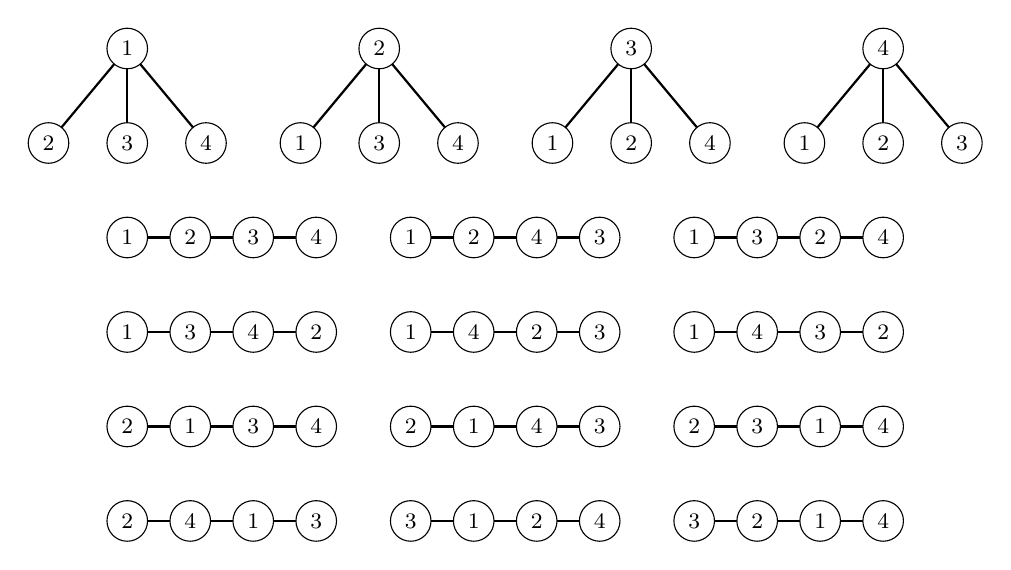
\begin{tikzpicture}[scale=0.8]
\footnotesize

\newcommand\puua[6]{
\path[draw,thick,-] (#1,#2) -- (#1-1.25,#2-1.5);
\path[draw,thick,-] (#1,#2) -- (#1,#2-1.5);
\path[draw,thick,-] (#1,#2) -- (#1+1.25,#2-1.5);
\node[draw, circle, fill=white] at (#1,#2) {#3};
\node[draw, circle, fill=white] at (#1-1.25,#2-1.5) {#4};
\node[draw, circle, fill=white] at (#1,#2-1.5) {#5};
\node[draw, circle, fill=white] at (#1+1.25,#2-1.5) {#6};
}
\newcommand\puub[6]{
\path[draw,thick,-] (#1,#2) -- (#1+1,#2);
\path[draw,thick,-] (#1+1,#2) -- (#1+2,#2);
\path[draw,thick,-] (#1+2,#2) -- (#1+3,#2);
\node[draw, circle, fill=white] at (#1,#2) {#3};
\node[draw, circle, fill=white] at (#1+1,#2) {#4};
\node[draw, circle, fill=white] at (#1+2,#2) {#5};
\node[draw, circle, fill=white] at (#1+3,#2) {#6};
}

\puua{0}{0}{1}{2}{3}{4}
\puua{4}{0}{2}{1}{3}{4}
\puua{8}{0}{3}{1}{2}{4}
\puua{12}{0}{4}{1}{2}{3}

\puub{0}{-3}{1}{2}{3}{4}
\puub{4.5}{-3}{1}{2}{4}{3}
\puub{9}{-3}{1}{3}{2}{4}
\puub{0}{-4.5}{1}{3}{4}{2}
\puub{4.5}{-4.5}{1}{4}{2}{3}
\puub{9}{-4.5}{1}{4}{3}{2}
\puub{0}{-6}{2}{1}{3}{4}
\puub{4.5}{-6}{2}{1}{4}{3}
\puub{9}{-6}{2}{3}{1}{4}
\puub{0}{-7.5}{2}{4}{1}{3}
\puub{4.5}{-7.5}{3}{1}{2}{4}
\puub{9}{-7.5}{3}{2}{1}{4}
\end{tikzpicture}
\end{center}
\end{samepage}

در ادامه بررسی می‌شود چگونه فرمول کیلی
با استفاده از کدهای پروفر اثبات می‌شود.

\subsubsection{کد پروفر}

\index{کد پروفر}

یک \key{کد پروفر}
%\footnote{In 1918, H. Prüfer proved Cayley's theorem using Prüfer codes \cite{pru18}.}
دنباله‌ای از
$n-2$ عدد است که یک درخت برچسب‌دار را توصیف می‌کند.
این کد طی فرایندی ساخته می‌شود
که در آن $n-2$ برگ از درخت حذف می‌شوند.
در هر مرحله، برگ با کوچک‌ترین برچسب حذف می‌شود،
و برچسب تنها همسایه آن به کد اضافه می‌گردد.

برای مثال، کد پروفر
گراف زیر محاسبه می‌شود:
\begin{center}
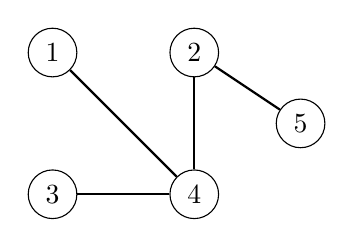
\begin{tikzpicture}[scale=0.9]
\node[draw, circle] (1) at (2,3) {$1$};
\node[draw, circle] (2) at (4,3) {$2$};
\node[draw, circle] (3) at (2,1) {$3$};
\node[draw, circle] (4) at (4,1) {$4$};
\node[draw, circle] (5) at (5.5,2) {$5$};

\path[draw,thick,-] (1) -- (4);
\path[draw,thick,-] (3) -- (4);
\path[draw,thick,-] (2) -- (4);
\path[draw,thick,-] (2) -- (5);
\end{tikzpicture}
\end{center}

ابتدا رأس 1 حذف شده و رأس 4 به کد اضافه می‌شود:
\begin{center}
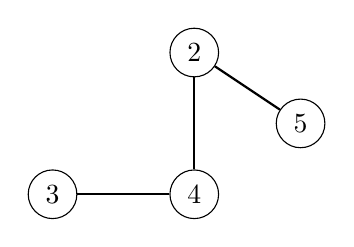
\begin{tikzpicture}[scale=0.9]
%\node[draw, circle] (1) at (2,3) {$1$};
\node[draw, circle] (2) at (4,3) {$2$};
\node[draw, circle] (3) at (2,1) {$3$};
\node[draw, circle] (4) at (4,1) {$4$};
\node[draw, circle] (5) at (5.5,2) {$5$};

%\path[draw,thick,-] (1) -- (4);
\path[draw,thick,-] (3) -- (4);
\path[draw,thick,-] (2) -- (4);
\path[draw,thick,-] (2) -- (5);
\end{tikzpicture}
\end{center}

سپس رأس ۳ را حذف و رأس ۴ را به کد اضافه می‌کنیم:
\begin{center}
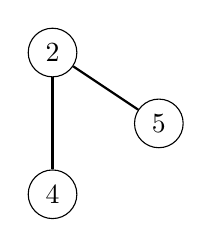
\begin{tikzpicture}[scale=0.9]
%\node[draw, circle] (1) at (2,3) {$1$};
\node[draw, circle] (2) at (4,3) {$2$};
%\node[draw, circle] (3) at (2,1) {$3$};
\node[draw, circle] (4) at (4,1) {$4$};
\node[draw, circle] (5) at (5.5,2) {$5$};

%\path[draw,thick,-] (1) -- (4);
%\path[draw,thick,-] (3) -- (4);
\path[draw,thick,-] (2) -- (4);
\path[draw,thick,-] (2) -- (5);
\end{tikzpicture}
\end{center}

در نهایت رأس ۴ را حذف و رأس ۲ را به کد اضافه می‌کنیم:
\begin{center}
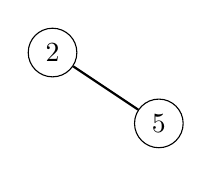
\begin{tikzpicture}[scale=0.9]
%\node[draw, circle] (1) at (2,3) {$1$};
\node[draw, circle] (2) at (4,3) {$2$};
%\node[draw, circle] (3) at (2,1) {$3$};
%\node[draw, circle] (4) at (4,1) {$4$};
\node[draw, circle] (5) at (5.5,2) {$5$};

%\path[draw,thick,-] (1) -- (4);
%\path[draw,thick,-] (3) -- (4);
%\path[draw,thick,-] (2) -- (4);
\path[draw,thick,-] (2) -- (5);
\end{tikzpicture}
\end{center}

بنابراین، کد پروفر گراف برابر $[4,4,2]$ است.

برای هر درخت می‌توان یک کد پروفر ساخت
و مهم‌تر آنکه،
درخت اصلی را می‌توان
از روی کد پروفر بازسازی کرد.
از این رو، تعداد درخت‌های برچسب‌دار
با $n$ رأس برابر است با
$n^{n-2}$، یعنی تعداد کدهای پروفر
به طول $n-2$ برای $n$ رأس.